\documentclass[pdflatex,compress,mathserif]{beamer}

%\usetheme[dark,framenumber,totalframenumber]{ElektroITK}
\usetheme[darktitle,framenumber,totalframenumber]{ElektroITK}

\usepackage[utf8]{inputenc}
\usepackage[T1]{fontenc}
\usepackage{lmodern}
\usepackage[bahasai]{babel}
\usepackage{amsmath}
\usepackage{amsfonts}
\usepackage{amssymb}
\usepackage{graphicx}
\usepackage{multicol}
\usepackage{framed}
\usepackage{minted}

\definecolor{LightGray}{gray}{0.95}

\usefonttheme[onlymath]{serif}

\newcommand*{\Scale}[2][4]{\scalebox{#1}{$#2$}}%

\setbeamertemplate{caption}[numbered]

\title{METODE NUMERIK}
\subtitle{Integral Numerik}

\author{Mifta Nur Farid}

\begin{document}

\maketitle

\begin{frame}{Integral Numerik}
    \begin{itemize}
        \item Integral = luas area di dalam kurva antara $a$ dan $b$
    \end{itemize}
    \begin{figure}
        \centering
        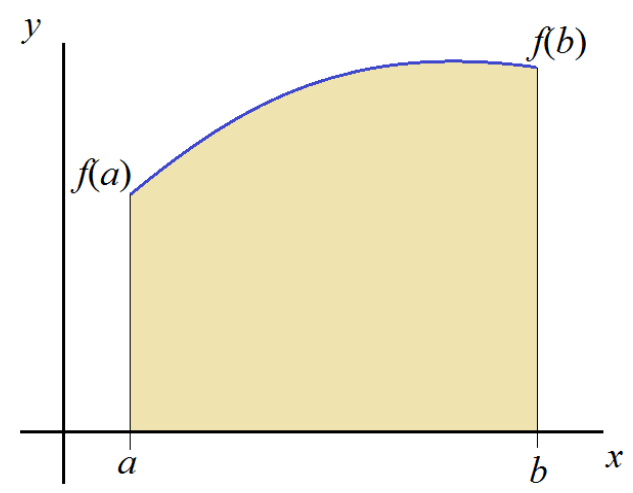
\includegraphics[width=0.7\linewidth]{./img/img01.png}
    \end{figure}
\end{frame}

\begin{frame}{Aturan Trapezoida}
    \begin{figure}
        \centering
        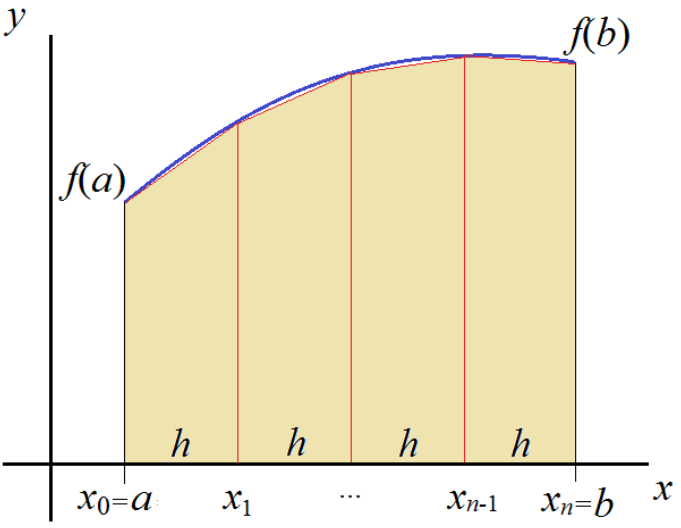
\includegraphics[width=0.6\linewidth]{./img/img02.png}
    \end{figure}
    \begin{itemize}
        \item Luas area pertama:
        \begin{figure}
            \centering
            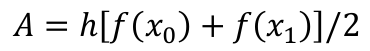
\includegraphics[width=0.4\linewidth]{./img/img03.png}
        \end{figure}
    \end{itemize}
\end{frame}

\begin{frame}{Aturan Trapezoida}
    \begin{itemize}
        \item Integral = total luas area trapezoida
    \end{itemize}
    \begin{figure}
        \centering
        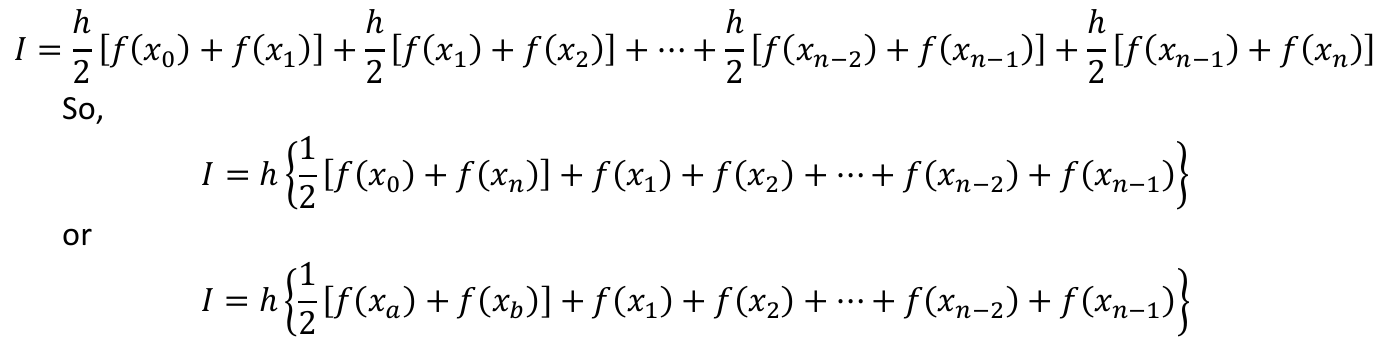
\includegraphics[width=\linewidth]{./img/img04.png}
    \end{figure}
\end{frame}

\begin{frame}{Aturan 1/3 Simpson}
    \begin{itemize}
        \item Lebih banyak garis
    \end{itemize}
    \begin{figure}
        \centering
        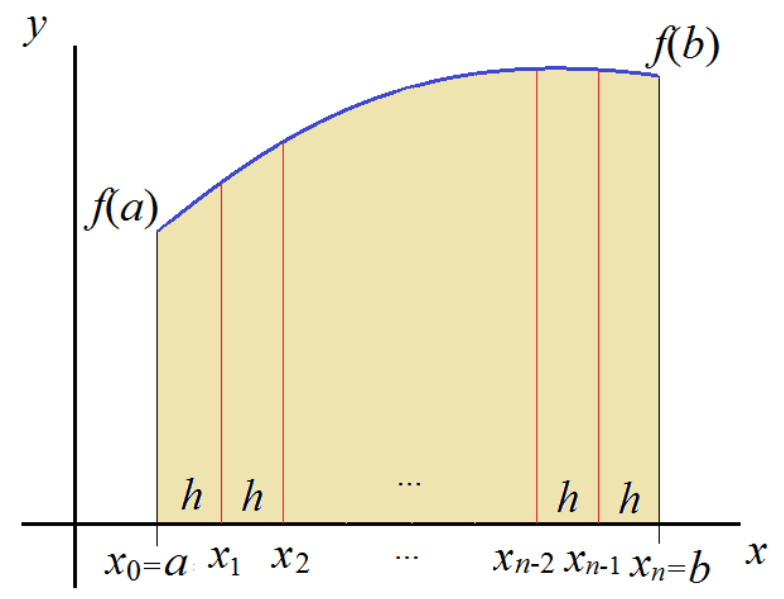
\includegraphics[width=0.6\linewidth]{./img/img05.png}
    \end{figure}
\end{frame}

\begin{frame}{Aturan 1/3 Simpson}
    \begin{itemize}
        \item Luasan pertama
        \begin{figure}
            \centering
            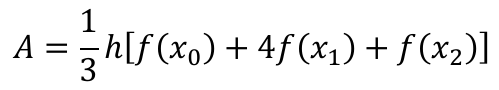
\includegraphics[width=0.6\linewidth]{./img/img06.png}
        \end{figure}
    \end{itemize}
    \begin{figure}
        \centering
        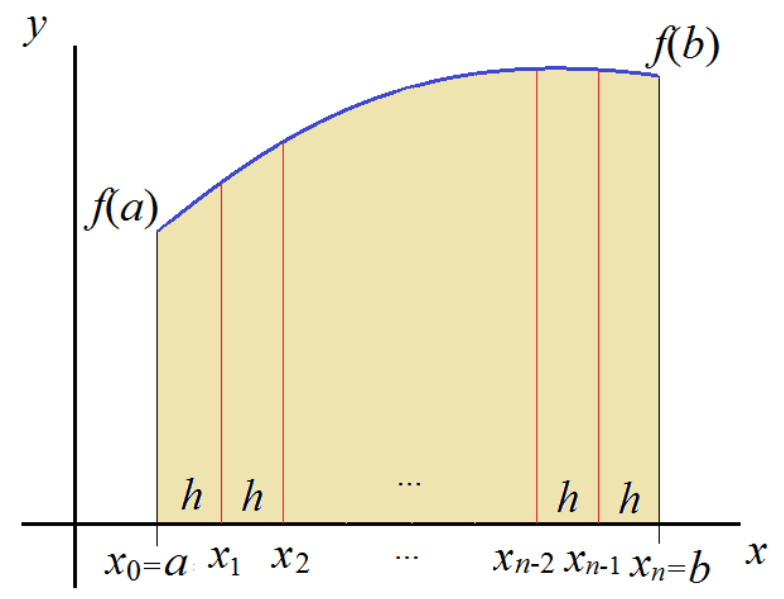
\includegraphics[width=0.6\linewidth]{./img/img05.png}
    \end{figure}
\end{frame}

\begin{frame}{Aturan 1/3 Simpson}
    \begin{itemize}
        \item Luas keseluruhan
    \end{itemize}
    \begin{figure}
        \centering
        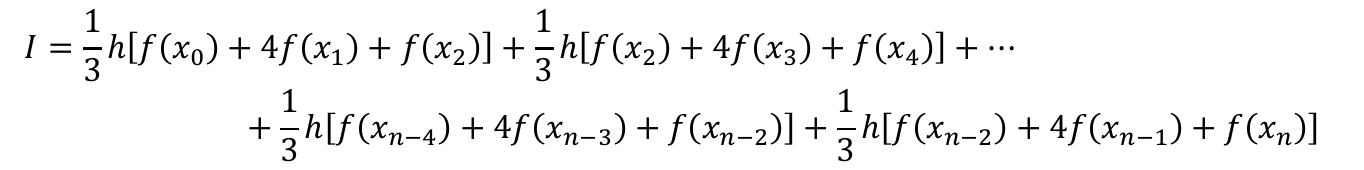
\includegraphics[width=\linewidth]{./img/img07.png}
    \end{figure}
\end{frame}

\begin{frame}{Aturan 1/3 Simpson}
    \begin{itemize}
        \item Bentuk yang lebih sederhana
        \begin{figure}
            \centering
            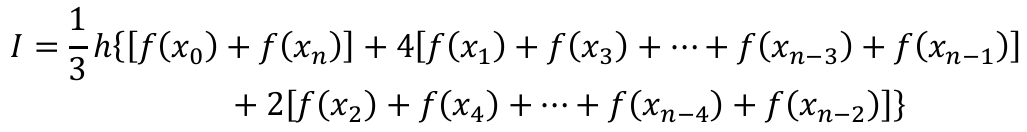
\includegraphics[width=\linewidth]{./img/img08.png}
        \end{figure}
        atau
        \begin{figure}
            \centering
            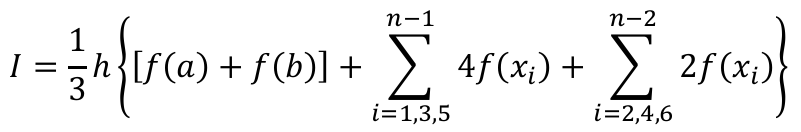
\includegraphics[width=\linewidth]{./img/img09.png}
        \end{figure}
    \end{itemize}
\end{frame}

\begin{frame}{Aturan 3/8 Simpson}
    \begin{itemize}
        \item Hitung 3 garis pertama, selanjutnya 4 garis.
        \item Persamaannya:
        \begin{figure}
            \centering
            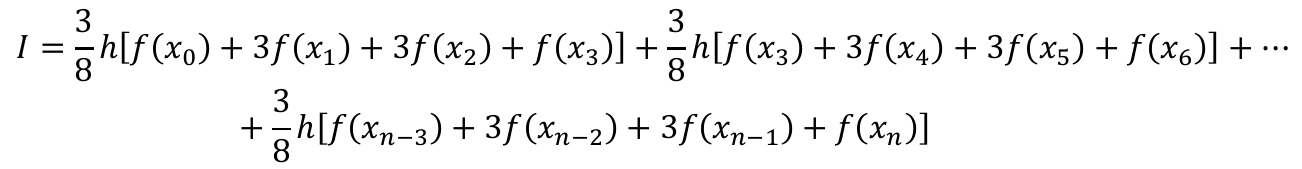
\includegraphics[width=\linewidth]{./img/img10.png}
        \end{figure}
        atau
        \begin{figure}
            \centering
            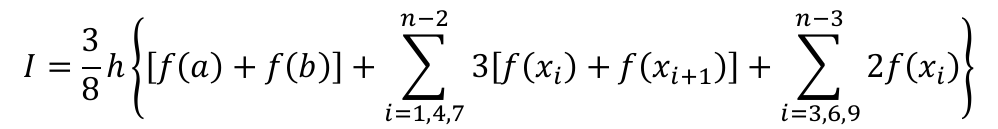
\includegraphics[width=\linewidth]{./img/img11.png}
        \end{figure}
    \end{itemize}
\end{frame}

\end{document}
